\documentclass[conference]{IEEEtran}
\usepackage{cite}
\usepackage{amsmath,amssymb,amsfonts}
\usepackage{algorithmic}
\usepackage{graphicx}
\usepackage{textcomp}
\usepackage{xcolor}
\usepackage{float}
\usepackage{tikz, pgfplots}
\usepackage{circuitikz}
\usepackage{booktabs}
\usepackage[english]{babel}
\usepackage[figurename=Fig.]{caption}
\usepackage[autostyle, english = american]{csquotes}

\usepackage{mathtools}
\usepackage{gensymb}
\usepackage{enumitem}
\MakeOuterQuote{"}
\def\BibTeX{{\rm B\kern-.05em{\sc i\kern-.025em b}\kern-.08em
    T\kern-.1667em\lower.7ex\hbox{E}\kern-.125emX}}

\pgfplotsset{compat=newest}

\begin{document}

\title{Autonomous Car Project\\

\author{\IEEEauthorblockN{Tevin Hendess}
\IEEEauthorblockA{\textit{Computer Engineering Department}\\
\textit{Rochester Institute of Technology}\\
Rochester, NY USA \\
twh4619@rit.edu}
\and
\IEEEauthorblockN{Adam Schultzer}
\IEEEauthorblockA{\textit{Computer Engineering Department}\\
\textit{Rochester Institute of Technology}\\
Rochester, NY USA \\
ajs1539@rit.edu}
}
}

\maketitle

\begin{abstract}
    The IDE Car Project is a legendary right of passage for RIT Computer
    Engineering students. Everything learned over the semester is combined
    with knowledge from previous coursework to create a fully autonomous
    vehicle. Provided with a standard vehicle frame, set of motors, servo,
    camera, and control board, the entire processes of programming and tuning
    the car is left up to the students. The process is done incrementally,
    beginning with small test milestones. Each of these ensures that the
    project is progressing smoothly and allows for changes to be made later in
    the process without fear that errors are from hardware or basic coding
    problems. The car is then entered into a time-trial race against other
    vehicles, all with the exact same frame and design constraints. At this
    point, only the code and tuning matter. Combining the multitude of
    different skillsets and knowledgebases required to get the car to function
    was an incredibly useful learning experience and tested students in a way
    that no project in Computer Engineering has before.
\end{abstract}

\section{Background and Description of Components}
    Important to understanding the car itself is understanding the design
    constraints and development process of the vehicle and the project as a
    whole. Each team began with a set of base components which were proven to
    be functional. These components are: a vehicle base, two drive motors,
    one servo motor, a line-scan camera, two batteries, an MSP-432P4111R
    microcontroller, and a motor controller.

    The total costs of all components are shown in Table \ref{tab:bom}.

    \begin{table}[htpb]
        \caption{Bill of Materials for All Required Components}
        \label{tab:bom}
        \centering
        \scalebox{0.9}{ % Adjust scale if needed
        \begin{tabular}{@{}lr>{\raggedright\arraybackslash}p{2.5cm}@{}}
        \toprule
        \textbf{Part} & \textbf{Price} & \textbf{Description} \\ 
        \midrule
        Vehicle Base & \$98.75 & ROB0170 \\ 
        TI MSP432P4111R & \$27.99 & TI MSP432P4111R Development Board \\ 
        Linker Board & provided & RPI Motor Driver and MSP432 Linker \\ 
        Motor Control Board & \$29.86 & MC33886 RPI Motor Driver Board \\ 
        Servo Motor & \$14.99 & Futaba S3004 \\ 
        DC Motor & \$43.90 & Two 12VDC 200RPM GHM-01 \\ 
        Line Scan Camera & \$105.95 & Parallax TSL-1401 \\ 
        Batteries & \$39.49 & Two Tenergy 7.2V 3800mAh NiMH batteries\\ 
        Battery Charger & provided & Charger for provided batteries \\ 
        Zip Ties & \$2.00 & -- \\ 
        OLED Display & \$15.00 & SSD1306 \\ 
        Bluetooth Module & \$15.00 & DSD-TECH HM-10 \\ 
        \bottomrule
        \end{tabular}
        }
        \end{table}

    The most basic of the provided components was a vehicle base. This was
    simply a metal frame onto which all of the electrical components could be
    attached. It contained axles and wheels with large gears which would be
    used to connect to the motors. The inclusion of gears was beneficial for
    a number of reasons. First, it allowed for the motors to be changed
    separately from the wheels and drive train itself. This isolated the two
    sections and meant that a failure in the motor didn't require replacing
    the wheels as well. The other benefit of gears was that the gear train
    allowed for an easy way to increase the torque output of the motor. The
    shaft of the motor was connected to a very small gear (12 teeth), while
    the axle for the wheels had a much larger gear (96 teeth). This meant that
    when the motor spun, the small gear would rotate eight times for every one
    revolution of the wheel. Such a gear ratio results in a much higher torque
    output on the wheel. The front wheels did not have gears as they were not
    directly powered. What they did have, however, were levers which permitted
    the wheels to turn while still spinning. This is the mechanism that the
    servo was connected to. The other notable parts of the base included
    numerous mounting points which allowed for the motors, servo, and
    electrical boards to be securely attached. The base also had a foam bumper
    in the front to avoid any shock to the circuitry if the car hit something.
    
    This frame was originally used for a similar competition which utilized
    control boards from a different manufacturer. The benefit of the frame's
    design is that it is modular, so the older boards could easily be removed
    and replaced with ones which were, at the time, still widely supported and
    available.

    The two drive motors were less complicated and simply required PWM signals
    to control their speed and power. These signals were programmed into the
    main microcontroller and then passed to the motor controller board to be
    properly translated into voltage values for the motors to understand. The
    two motors were controlled independently to allow for differential
    driving. Including this meant that when turning, the motor on the same
    side as the turn would rotate backwards, similar to how a tank would spin
    by driving its treads in opposite directions. Such functionality was
    incredibly useful as it greatly decreased the turning radius required for
    the car to navigate corners. This would not have been possible without
    independent control of the motors.

    The servo motor was the main method by which the car turned and followed
    the track, as opposed to differential drive which was only a supporting
    feature and could not turn the entire car on its own. By sending a
    position to the servo, the front wheels could be commanded into any angle.
    It was imperative that the servo be fast enough to switch continuously
    between different turning directions to get past the "snake" parts of the
    course. The holding power was also important as the servo would have to be
    able to resist the force from the track as the wheels turned and held
    through the car's high-speed maneuvering.

    The line-scan camera is the only external sensor on the car and is what
    gives the vehicle its autonomous capability. When pointed at a section of
    track (designed with two black lines surrounding a solid white center),
    the camera outputs a single 128 bit line of information about the current
    light level at each point. A sample output from the camera is shown in
    Fig. \ref{fig:camera_graph}. When viewing an image with clear contrast
    like that of the track pieces, the camera can be used to get a clear idea
    of where the edges are. The bottom graph in Fig. \ref{fig:camera_graph}
    labeled "Binary Conversion" is what the analog to digital convertor (ADC)
    on the microcontroller outputs and was originally used for controlling the
    car. At the last minute, the design shifted to use the "Smoothed Voltage"
    information instead.

    The batteries provided the electrical power for the motors, servo, camera,
    and controlling circuitry on the car. While relatively simple devices, the
    voltage level of the batteries could have a measurable impact on the
    performance of the car. While rated for 7.6 volts, the batteries could
    range from anywhere between about 7V to nearly 8V5 depending on the charge
    level. The car's motors would perform better at higher voltages, so care
    was taken to ensure that the batteries were nearly fully charged before
    important tests and that any tuning was done at a known voltage. Tuning
    values for voltages which wouldn't end up being used in the race would
    have been a waste of time.
    
    The motor controller and MSP432 are where all of the electrical signals
    were generated and contained the program which tied everything together.
    The input from the camera provided the controller with knowledge of the
    track ahead. With this information and control algorithms, it would then
    decide where the front wheels needed to turn and in what direction and
    speed the back tires had to spin. This information was sent to the motor
    controller board which then translated the commands into PWM control
    signals which would affect the required outcome on the drivetrain. The
    motor controller was also responsible for stepping down the voltage from
    the battery to a level that the MSP432 was able to run at.

    All of these components combined to form a vehicle which could take in
    information about the world around it, make decisions based on that
    information, and then execute an action. It was important, however, to
    ensure that each component was working as expected before serious effort
    could be devoted to tuning anything. To this end, the milestones focused
    on verifying the hardware, proving line-following code, testing turns and
    intersections, and finally implementing PID control and variable speed.
    At each step in this process, the challenges became more and more complex.
    By the time the final milestone was completed, however, the only work left
    was tuning the control values to the exact lighting conditions of the
    competition space. There were also some additional bonus features which
    could be added later.

    Because of how the milestones were laid out, passing one step meant that
    completing the next step would be entirely dependent on new code added
    rather than the possibility that something earlier on was broken. For
    example, testing all of the hardware to start off ensured that if the car
    randomly drove to the left, it was likely a result of the code powering
    the right motor too strongly and not because the servo had random
    twitches. Of course, some problems with hardware still arose, but any
    early ones were caught through the milestone testing.

    As a final step once the car was running, additional features could be
    added to improve functionality, prepare for extra obstacles, or gain bonus
    points. Functionality improvements included the aforementioned
    differential drive which reduced turning radii. Additionally, some time
    was devoted to preparing for the possibility that a tunnel piece would be
    added to the track. Unlike the swiggles or ramp, the tunnel altered the
    light level on the track and presented a very formidable obstacle. While
    some brainstorming was done as to how this impact could be mitigated, it
    was determined that the piece would be too disruptive to be introduced
    late in the development cycle and the choice was made to focus efforts
    elsewhere. As a final possibility, a "line-stopping" routine could have
    been implemented which would automatically stop the car once it had
    completed one lap. This was determined by a dashed line drawn
    perpendicularly across the starting track piece. Correct stopping
    functionality came with the bonus of one section removed from the car's
    final time. While such an offer is tantalizing, attempts to implement
    this feature were unsuccessful. The main reason for this failure was the
    difficulty of testing the line-stopping in the practice space. Because the
    pieces had to be moved and were not taped down, many gaps formed in
    between them as different teams tested their algorithms. This meant that
    there was a high likelihood of the line-stopping routine mistakenly
    stopping the car before the finish line, so it was abandoned.

    \begin{figure}[h]
        \centering
        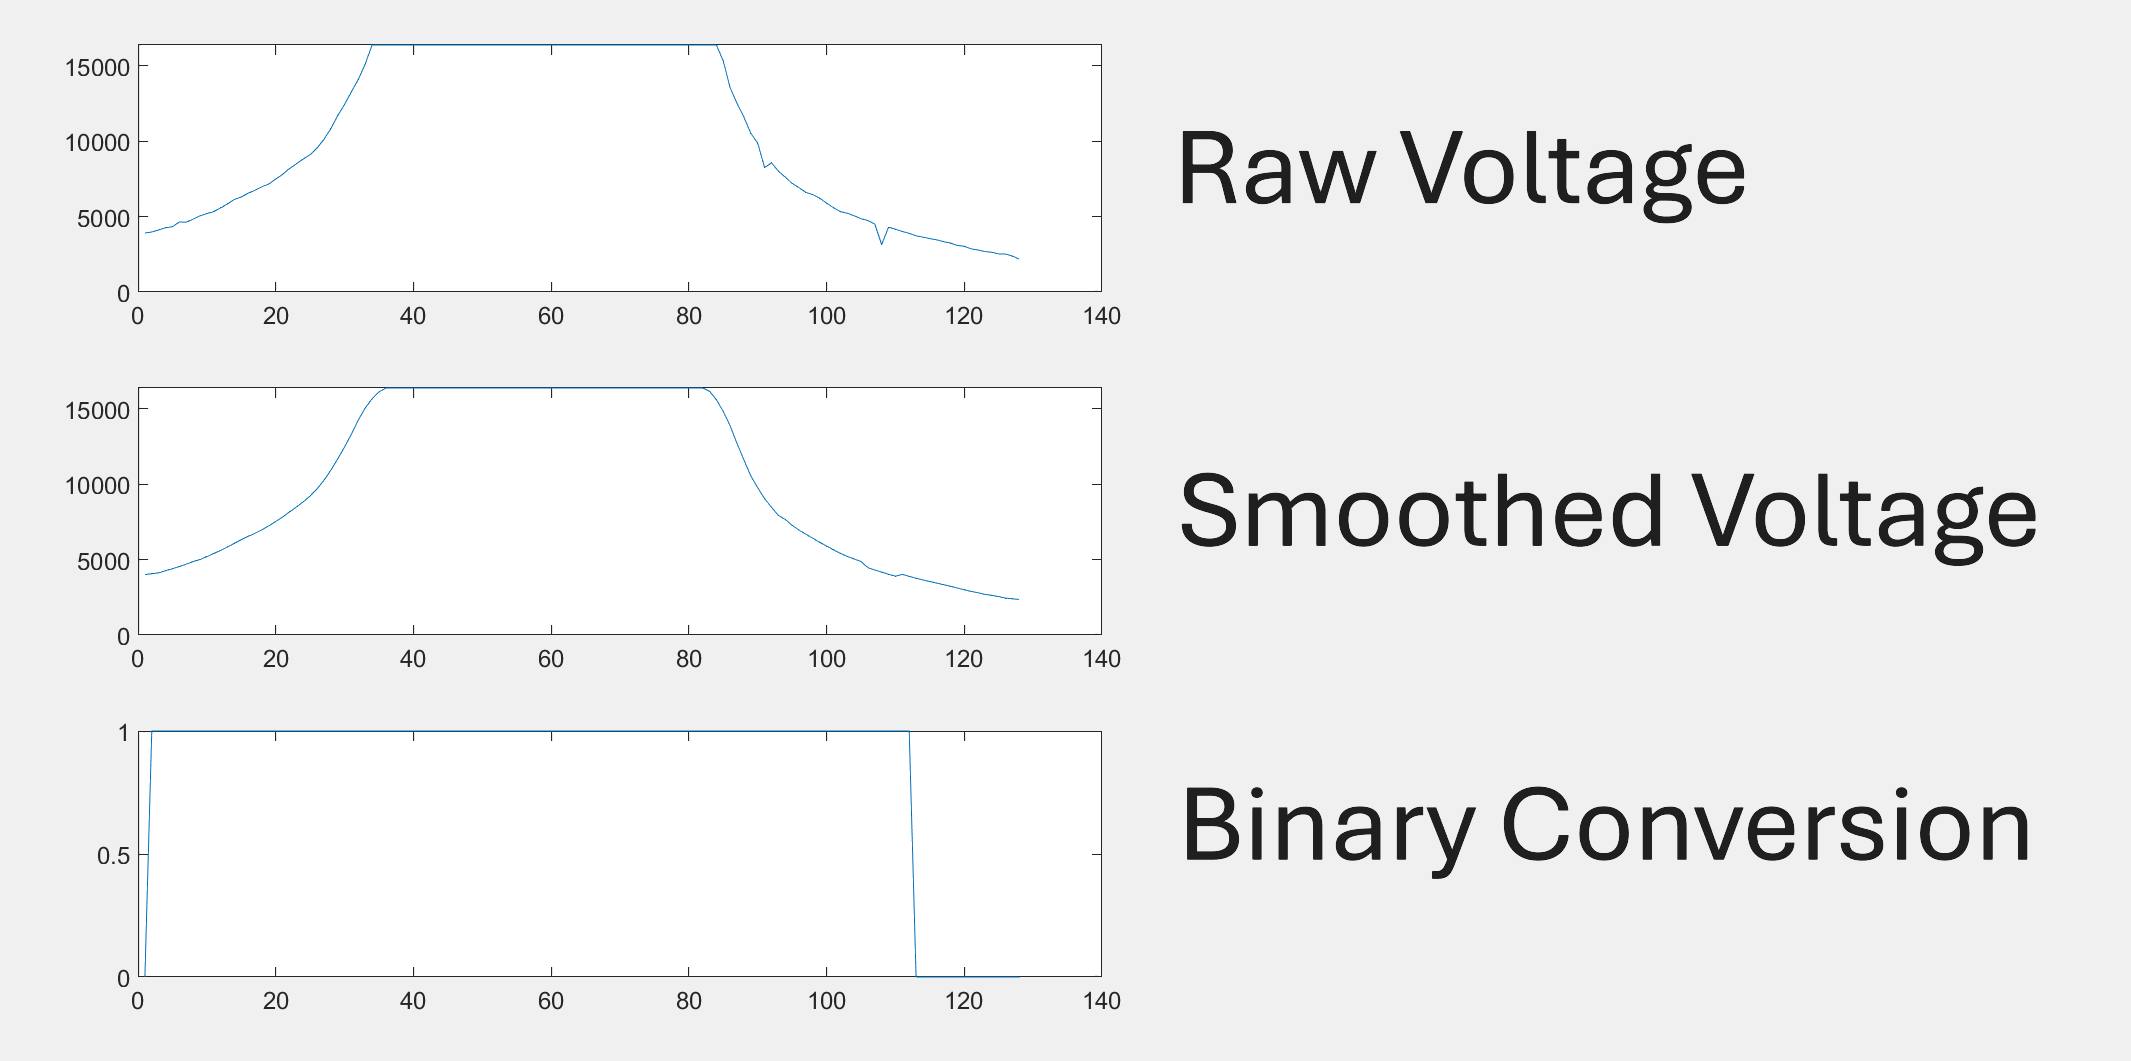
\includegraphics[width=\linewidth]{{images/part3matlab.png}}
        \caption{MatLab Graphs of Sample Camera Ouput}
        \label{fig:camera_graph}
    \end{figure}
    
\section{Design of Circuits}

\section{Description of Algorithms}

\section{Hardware Bill of Materials}

\section{Key Challenges and What Could be Improved}

\section{Conclusion}

%COMMENTED CODE IS ALSO REQUIRED

\begin{thebibliography}{00}
    \bibitem{b1} 
    \end{thebibliography}

\end{document}
